\documentclass[11pt]{article}
% Эта строка — комментарий, она не будет показана в выходном файле
\usepackage{ucs}
\usepackage[utf8x]{inputenc} % Включаем поддержку UTF8
\usepackage[russian]{babel}  % Включаем пакет для поддержки русского языка
\usepackage{amsmath}
\usepackage{mathtools}
\usepackage{amssymb}
% \usepackage[dvips]{graphicx}
% \graphicspath{{noiseimages/}}
\usepackage[pdftex]{graphicx}


% Параметры страницы: 1см от правого края и 2см от остальных.


\hoffset=0mm
\voffset=0mm
\textwidth=180mm        % ширина текста
\oddsidemargin=-6.5mm   % левое поле 25.4 - 5.4 = 20 мм
\textheight=240mm       % высота текста 297 (A4) - 40
\topmargin=-15.4mm      % верхнее поле (10мм)
\headheight=5mm      % место для колонтитула
\headsep=5mm          % отступ после колонтитула
\footskip=8mm         % отступ до нижнего колонтитула


\begin{document}
    \author {Зотов Алексей 496 гр.}
    \title {Лабораторная работа 1.1 \\  Определение скорости полета пули при помощи баллистического маятника}
    \maketitle{}   

    \indent
    \textbf{Цель работы:} определить скорость полета пули, применяя законы сохранения и используя баллистический маятник, познакомиться с базовыми принципами обработки экспериментальных данных.
    \\ 
    \indent
    \textbf{В работе используются:} духовое ружье на штативе, осветитель, оптическая система для измерения отклонений маятника, измерительная линейка, пули и весы для их взвешивания, баллистический маятник.


    \small{
    Для измерения переданного пулей импульса и, следовательно, ее скорости используют баллистический маятник. Баллистическим называется маятник, колебания которого вызываются кратковременным начальным импульсом (толчком). Кратковременным можно считать импульс, если время действия сил (время соударения) значительно меньше периода колебаний маятника. При этом отклонение маятника за время соударения значительно меньше амплитуды колебаний.}

    \begin{center} 
        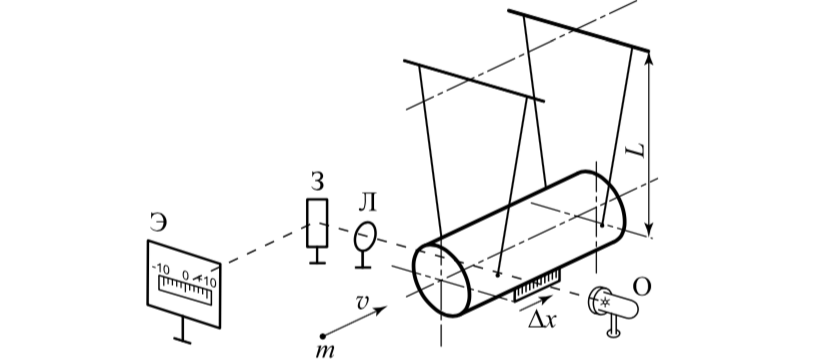
\includegraphics[width=4in , height = 1.5in]{ust.png} \\ Рис. 1: Схема установки для измерения скорости полета пули
    \end{center}


    \small{
    Используемый в этой работе баллистический маятник представляет собой тяжелый цилиндр, подвешенный на четырех нитях одинаковой длины. Он изображен на рис. 1 вместе с измерительной системой. Важной особенностью используемой системы подвески маятника является то, что при колебаниях ось цилиндра перемещается параллельно самой себе без вращения. Колебания происходят так, как будто вся масса маятника сосредоточена в его центре масс. Любая точка цилиндра при колебаниях маятника движется по дуге окружности, радиус которой равен расстоянию по вертикали между уровнями верхнего и нижнего концов нитей подвеса.
    \\
    \indent Связь между максимальным отклонением маятника и начальной скоростью, полученной им в результате толчка, описывается законом сохранения механической энергии, если потери энергии за период значительно меньше энергии его колебаний. По начальному максимальному отклонению маятника определяются импульс и скорость пули.
    \\
    \indent Внешними силами для системы пуляцилиндр являются сила тяжести, которая не имеет горизонтальной компоненты, и силы натяжения нитей, у которых появляются горизонтальные компоненты при отклонении маятника. Однако если отклонения малы, то и эти компоненты малы. Тем более мал по сравнению с импульсом пули их импульс за время соударения. Поэтому закон сохранения импульса при соударении пули с цилиндром имеет вид :
    }
    \begin{equation}
        mu = (M + m) V   
    \end{equation}
    Здесь $m$ — масса пули, $M$— масса цилиндра, $u$ — скорость пули перед ударом, $V$ — скорость цилиндра и пули после неупругого соударения.\\
    \indent Учитывая, что масса маятника значительно больше массы пули, можно написать :
    \begin{equation}
        u = \frac{M}{m}V   
    \end{equation}

    \indent Получив начальную кинетическую энергию, маятник при отклонении будет подниматься до тех пор, пока всю ее не израсходует. Если пренебречь потерями, то вся кинетическая энергия переходит в потенциальную в поле тяжести. Тогда по закону сохранения механической энергии высота $h$ подъема маятника над его начальным положением связана с начальной скоростью маятника $V$ следующим образом:
    \begin{equation}
        V^2 = 2gh   
    \end{equation}
    \indent Высота подъема маятника выражается через угол $\varphi$ отклонения маятника от вертикали:
    \begin{equation}
        h = L(1 - \cos\varphi) = 2L\sin^2\frac{\varphi}{2}, \quad \text{где } \varphi \approx \frac{\Delta x}{L}  
    \end{equation}
    Считая $\varphi \ll 1$ , получаем окончательную формулу для определения скорости пули:
    \begin{equation}
    u = \frac{M}{m} \sqrt{\frac{g}{L}}\Delta x
    \end{equation}

    \textbf{Ход работы}
    \begin{enumerate} 
    \item \underline{Измерение массы пуль.} \\
        \indent Измерим на аналитических весах суммарную массу всех пулек, а также массу каждой пульки в отдельости:
        $M_{all} = 4.154$[g] \\

        \begin{table}[h]
                    \caption{Масса пуль.}
                    \begin{center}
                    \begin{tabular}{|c|c|c|c|c|c|c|c|c|}
                            \hline 
                                $i$ & 1 & 2 & 3 & 4 & 5 & 6 & 7 & 8 \\
                            \hline
                                $m_i , [g]$ & 0.516& 0.515& 0.520& 0.524& 0.527& 0.511& 0.523& 0.516\\
                            \hline
                            \end{tabular}
                        \end{center}
        \end{table}

        Среднее значение массы пульки : $m_{cp} = 0.519$
        Cреднеквадратичное отклонение масс пулек от среднего значения : $\sigma_{m} = 0.005$


        Проверим аддитивность массы: $M^*_{all} = \Sigma m_{i} = 4.152$ , $\Delta M = |M^*_{all} - M_{all}| = 0.002$, погрешность одного измерения $\Delta m = 0.0005 \implies$ погрешность результата $\Delta_M = m * 8 = 0.004$. Можно говорить о выполнении закона аддитивности массы.

    \item \underline{Параметры установки.} \\
        Масса маятника $M = 2900 \pm 5$ [g]. \\
        $L = 225 \pm 0.5$ [cm].
    \item \underline{Измерение отклонений.}
        Произведем 8 выстрелов, $i$-му выстрелу соответствует пуля с номером $i$.
        \begin{table}[h]
                    \caption{Отклонение от положения равновесия.}
                    \begin{center}
                    \begin{tabular}{|c|c|c|c|c|c|c|c|c|}
                            \hline 
                                $i$ & 1 & 2 & 3 & 4 & 5 & 6 & 7 & 8 \\
                            \hline
                                $\Delta x_i = x_i - x_0 , [mm]$ &15&17&16&14&15&14&14&15\\
                            \hline
                            \end{tabular}
                        \end{center}
        \end{table}

        \indent $\sigma_{x_0} = 0.2 $ [mm]  \\
        \indent $\sigma_{x_i} = 1.5 $ [mm]  \\
        \indent $\sigma_{\Delta x_i} \approx 1.5 $ [mm]

    \clearpage{}
    \item \underline{Определение скорости пули.} \\
        Для определения скорости пули воспользуемся формулой (5): \\
        \begin{table}[h]
                    \caption{Скорость пули.}
                    \begin{center}
                    \begin{tabular}{|c|c|c|c|c|c|c|c|c|}
                            \hline 
                                $i$ & 1 & 2 & 3 & 4 & 5 & 6 & 7 & 8 \\
                            \hline
                                $v_i , [m/c]$ &176&200&186&162&172&166&162&176 \\
                            \hline
                            \end{tabular}
                        \end{center}
        \end{table}    
        
        Среднее значение скорости: $v_{cp} = 175$ [m/c] \\
        Cреднеквадратичное отклонение скоростей от среднего значения: $\sigma_{v_{cp}} \approx 12$ [m/c]

        Погрешность каждого измерения вычислим по формуле : 
            $\sigma_{v_i} = \sqrt{\sigma^2_{L}(v_i) + \sigma^2_{\Delta x_i}(v_i) + \sigma^2_{m_i}(v_i)}$ , 
            где $\sigma_{x}$ - отклонение, вызванное погрешностью величины $x$.
        \begin{table}[h]
                    \caption{Погрешность скорости пули для каждого измерения.}
                    \begin{center}
                    \begin{tabular}{|c|c|c|c|c|c|c|c|c|}
                            \hline 
                                $i$ & 1 & 2 & 3 & 4 & 5 & 6 & 7 & 8 \\
                            \hline
                                $\sigma_{v_i} , [m/c]$ &17.7&17.8&17.6&17.5&17.4&17.9&17.5&17.7\\
                            \hline
                            \end{tabular}
                        \end{center}
        \end{table}    
        \\
        
        Посмотрим на вклады погрешностей в отдельности:

        \begin{table}[h]
                    \caption{Составляющие погрешности скорости пули для каждого измерения.}
                    \begin{center}
                    \begin{tabular}{|c|c|c|c|c|c|c|c|c|}
                            \hline 
                                $i$ & 1 & 2 & 3 & 4 & 5 & 6 & 7 & 8 \\
                            \hline
                                $\sigma^2_{\Delta x_i}(v_i) , [m/c]$ 
                                &314.6&315.8&309.7&305.0&301.6&320.7&306.2&314.6\\
                            \hline
                                $\sigma^2_{L}(v_i) , [m/c]$  &0.0&0.0&0.0&0.0&0.0&0.0&0.0&0.0 \\
                            \hline
                                $\sigma^2_{m_i}(v_i) , [m/c]$ &0.2&0.2&0.2&0.2&0.2&0.2&0.2&0.2 \\
                            \hline
                            \end{tabular}
                        \end{center}
        \end{table}


        Из таблицы можно видеть, что наибольший вклад в погрешность результата привносит погрешность измерения отклонения. Из - за этого погрешность каждого измерения превосходит среднеквадратичное отклонение результата от среднего. Отсюда можно сделать вывод, что сильные различия полученных скоростей вызваны, в основном, именно погрешностью измерения отклонения, а не реальным различием скорости от выстрела к выстрелу.

    \end{enumerate}
\end{document}